\chapter{Vehicle Platform}
The development of the Research Concept Vehicle started in 2012. The resulting electric two-seater is equipped with four autonomous cornering modules, that enable it to actuate each wheel independently with respect to steering angle, camber, driving or braking forces. Weighing around 400 kilogram the car can be driven one hour under normal conditions and reaches speeds of up to 70 kilometers per hour. Due to the fact that actuators are controlled by wire rather than mechanically it opens up a whole suit of new capabilities, that can improve handling, efficiency as well as safety.

The uniqueness of the platform makes it more relevant than ever for the quest of finding future mobility solutions. The interest for the platform even extended as far as the USA. Zoox Inc. a company based in the Silicon Valley developing self-driving taxis was in search for a platform to develop their cars on, as they decided that they would not want to develop a car from scratch. With the goal to build in redundancy and develop as little parts as possible the choice for the RCV was quickly made, providing a a car with four equal corner modules allowing multi-directional driving \cite{Harris.2015}.

\begin{figure}[h]
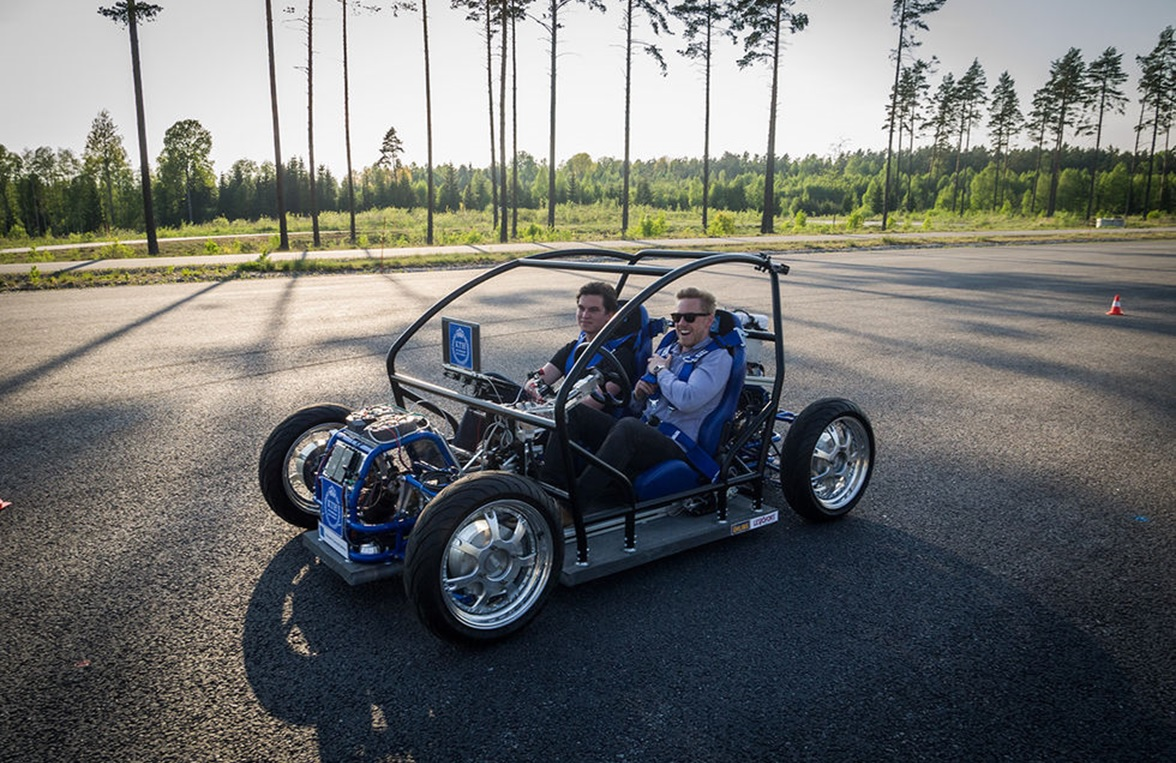
\includegraphics[width=\textwidth,trim={0 2.5cm 0 3.5cm},clip]{RCV.jpg}
\caption[Research Concept Vehicle of the ITRL]{Research Concept Vehicle of the Integrated Transport Research Lab}
\label{fig:RCV}
\end{figure}
